\documentclass{sig-alternate}
\usepackage{graphicx}
\usepackage{amsmath}
\usepackage{amssymb}
\usepackage{natbib}
\usepackage{myAlgorithm}

\bibliographystyle{abbrvnat}


%XXX:  Machine Learning for Auto-tuning: A Data-Drive Approach...} ???
\title{Boosted Regression Trees for Data-Driven Auto-Tuning}

\numberofauthors{3}

\author{
%\alignauthor First Last\titlenote{}\\
\alignauthor First Last\\
\affaddr{Affiliation line 1}\\
\affaddr{Affiliation line 2}\\
\email{anon@mail.com}
% 2nd author
%\alignauthor First Last\titlenote{None}\\
\alignauthor First Last\\
\affaddr{Affiliation line 1}\\
\affaddr{Affiliation line 2}\\
\email{anon@mail.com}
% 3rd author
%\alignauthor First Last\titlenote{None}\\
\alignauthor First Last\\
\affaddr{Affiliation line 1}\\
\affaddr{Affiliation line 2}\\
\email{anon@mail.com}
}

\begin{document}
\maketitle

\begin{abstract}
Auto-tuning is a widely used and effective technique for optimizing a
parametrized GPU code template for a particular computation on particular
hardware.  Its drawback is that thorough or exhaustive auto-tuning requires
compiling many kernels and calling each one many times; this process is slow.
Furthermore, library abstraction boundaries provide operations such as image
filtering and matrix multiplication, which actually correspond to a large set
of potential problem configurations with a wide variety of memory access
patterns and computational bottlenecks.  How can we draw on data from previous
empirical auto-tuning of related problems on related hardware to make a just-in-time
implementation decision for a novel problem?  This paper presents a machine
learning approach to auto-tuning, in which features of (a) the current
hardware platform, (b) the kernel configuration and (c) the problem instance
are passed to a regression model (boosted regression trees) which predicts how
much faster this kernel will be than a reference baseline.  Combinatorial
optimization strategies that would normally implement auto-tuning by
evaluating kernel configurations on the real hardware are orders of magnitude
faster when evaluating the surrogate regression model instead.  We validate our approach
using the filterbank correlation kernel described in \citet{pinto+cox:2011gcg}, where we find
that 0.1 seconds (XXX) of hill climbing on the regression model ({\em
predictive}
auto-tuning) can achieve an
average of 95\% of the speed brought by 120 seconds of empirical auto-tuning XXX.  Our
approach is not specific to filterbank correlation, or even to GPU
kernel auto-tuning: the approach of using a non-linear regression model on top of
simple features applies to a variety of problem types, kernel types, and
platforms.
\end{abstract}

\section{Introduction}

There is a natural function from
problem space x implementation space x platform space to runtime:
how much wall time elapses on the given platform when solving the given
problem with the given implementation.

Auto-tuning is a family of empirical techniques for finding the implementation
that minimizes that runtime function, when the platform and the problem
configuration are given.

XXX: some math, or possibly a picture with the three boxes that was on Pinto's
whiteboard.

This paper is about different ways of doing the minimization.
For a particular problem (filterbank correlation) we
look at a parameterized kernel implementation (from GCG)
and a few hardware platforms, and compare
random search, grid search, and a hill-climbing strategy with a good, but
generic, reference implementation.
Then we show that we can model the LSM function with a regression tree
well enough to usefully perform the argmin of Equation~\ref{eq:lsm_argmin}
on the model rather than the actual system. Whereas it may take several
minutes to perform a hill-climbing or grid search in the original system,
a hill-climbing search in the model requires a small fraction of a second.
Model-based autotuning makes it possible to simulate auto-tuning quickly and
accurately enough to be used within a single library call of the computational
routine.

\cite{volkov+demmel:2008}
\cite{vuduc:2003} % has some stuff about ML for autotuning in ch. 9


\subsection{Filter-bank Correlation}

Following [XXX], the experiments in this paper will focus on filterbank
correlation.  Mathematically, we define filterbank correlation in terms of an
image $x$ and a filterbank $f$.
The image $x$ has $R$ rows, $C$ columns, and $D$ channels (e.g. color
channels) that we call its {\em depth}. We index $x$ like $\mathbf{x}[i,j,d]$
where $0 \leq i < R$, $0 \leq j < C$, and $0 \leq d < D$.
The filterbank $f$ has $F$ filters that are like little images: each has a
height $H$, a width $W$, and $D$ channels.
We will restrict ourselves to what are called {\em valid} correlations, in
which the image is larger in both rows and columns than the filters.
The result of filterbank correlation of $x$ with $f$ is an image-like array
$z$ with $R-H+1$ rows, $C-W+1$ columns, and depth $F$, whose elements are
defined according to Equation~\ref{eq:z}:

\begin{equation}
    \mathbf{z}[r,c,k] = \sum_{w=0}^{W-1} \sum_{h=0}^{H-1} \sum_{d=0}^{D-1}
        \mathbf{x}[r+h, c+h, d]~ \mathbf{f}[k, h, w, d].
        \label{eq:z}
\end{equation}

Filterbank correlation is used extensively in image and video processing,
where it is often the computational bottleneck.
GPUs are well-suited to computing filterbank correlations, although the
optimal strategy for doing so often depends on the shape of the problem, i.e.
the choices of $R$, $C$, $D$, $F$, and $W$.
The computation of filterbank correlation on GPUs was recently treated by
\citet{pinto+cox:2011gcg}, which serves as the basis for the present work.

In terms of floating point operations, a filterbank correlation requires the
inner sums to be computed for each output pixel, yielding the quantity in
Eq.~\ref{eq:flops}:
\begin{equation}
\mathrm{FLOPS} = 2  K  H  W  D  (R - H + 1)( C- W + 1)
\label{eq:flops}
\end{equation}
The multiplicative factor of 2 arises because we must multiply an element of
$x$ with an element of $f$ and then add the result to an element of $z$.

In terms of bandwidth, if we were to assume (optimistically) that the entire
filterbank fit into the GPU's so-called constant memory, then the bandwidth
required for a filterbank correlation would be the size of the filterbank,
plus the size of the input image, plus the size of the output image. This sum
is expressed in terms of configuration parameters in Eq.~\ref{eq:bytes}:
\begin{align}
\mathrm{Bytes} = 4&RCD \nonumber \\
& + 4KHWD \nonumber \\
& + 4(R-H+1)(C-W+1)K
\label{eq:bytes}
\end{align}
We will see the bandwidth requirements of a more realistic analysis in
Section~XXX.

XXX: TYPICAL OF STENCIL COMPUTATIONS.

``Although the auto-tuning strategy has been successfully applied to libraries,
generalized stencil kernels are not amenable to packaging as libraries.''
\cite{kamil+etal:2009}


\cite{datta:2009}


\section{Configuration Spaces}

Recall from the introduction (Eq.~\ref{eq:condopt}) that we are addressing a
conditional optimization problem, in which we condition on a problem
configuration ($P$) and a system specification ($S$), and search for the best
implementation $I$ for addressing problem $P$ on system $S$.
This section describes the configuration spaces we used in our tests,
which are described later in Section XXX.


\subsection{Problem Description Space}

Mathematically, filterbank correlation is an operation on an $R \times C \times
D$ image and a $F \times H \times W \times D$ filterbank.
We randomly sampled problem specifications from the following space:
\begin{align*}
R = C & \in \{ 256, 512, 1024, 2048, 4096 \} \\
H = W & \in \{ 3, 5, 7, 9, 11 \} \\
D &  \in \{1, 4, 8, 16, 32, 64, 128, 256 \} \\
F &  \in \{1, 4, 8, 16, 32, 64, 128, 256 \}
\end{align*}
The product space
includes 1600 elements, but we restricted our experiments to problems that
represented between 1 and 50 gigaflops. Our problem space included 602
configurations. A library implementation that must support all image and
filter sizes must handle on the order of $2^{50}$ forseable
problem configurations (not even including variations due to strided memory
layouts).

%XXX: DIAGRAM OF IMAGE, FILTERBANK, OUTPUT

% Problems were considered invalid if the filters were larger than the images.
% but in the new setting with iheight >= 256 this never happened.
Problems were tested if they represented between 1 and 50 gigaflops.  Problems
that were smaller do not fully utilize the hardware, and are handled equally
well by many kernel settings.
Problems that were larger take so long to evaluate that there is negligible
inefficiency in implementing them via multiple calls with smaller images and fewer filters.
The configuration space described in Figure~\ref{fig:probspace} included 602
configurations with between 1 and 50 gigaflops.

In a full, reusable, library implementation of the filter correlation
operation, we would also provide options for arbitrary image shapes,
arbitrary integer depth and filter shapes, and also support a variety of
physical input layouts via strides.  These additional options would make our
approach of automatic auto-tuning even more important, because there would be
a greater variety in the kinds of computations and memory transfers to
perform.


\subsection{Implementation Description Space}

The strategy we use for computing filterbank correlation on the GPU
using CUDA follows \citet{pinto+cox:2011gcg}.
The overall strategy is to load the filterbank into constant memory, which is
relatively fast and visible to all threads, and then launch a grid of blocks
that tiles the output image.
Each thread computes $4 \times n\_output\_4s$ channels for some column and row of $z$.
Each block computes $4 \times n\_output\_4s$ channels for a subrectangle of the output image ($z$).
When there are more than $4 \times n\_output\_4s$ channels in $z$, or if the
filterbank is too large to fit into constant memory, then multiple
kernel executions perform the full computation.
Our approach permits splitting the filterbank along
the number-of-filters dimension ($F$) and the height dimension ($H$).
All the filterbanks in our study are small enough that
at least one row of a single filter can fit into constant memory.
Pseudo-code for the kernel is given in Figure~\ref{fig:kernel}.

\begin{figure}[!ht]
\centerline{
\begin{algorithm}{$\Algo{fbcorr}\big(gX, cF, gZ \big)$}
\Aitem shared $sX \setto$ all channels of region ($\beta$) of $gX$
\Aitem $x, y \setto$ position of this thread in output image
\Aitem \_\_syncthreads()
\Aitem $v[0:N] \setto 0$, for $N=4\times n\_output\_4s$
\Aitem for $d \setto 0$~\To~$D$,
\Aitem ~ for $h \setto 0$~\To~$H / n\_filter\_r$,
\Aitem ~ ~ for $w \setto 0$~\To~$W$,
\Aitem ~ ~ ~ $u \setto sX[x+h, y+w, d]$
\Aitem ~ ~ ~ for $n \setto 0$~\To~$n\_output\_4s - 1$,
\Aitem ~ ~ ~ ~  $v[n] \setto v[n] + cF[n, h, w, d]$
\Aitem for $n \setto 0$~\To~$n\_output\_4s - 1$,
\Aitem ~  gZ[x][y][4n:4n+n] += v[4n:4n+n], (float4)
\end{algorithm}
}
\caption{Kernel pseudo-code for filterbank correlation.
Input $gX$ is a pointer to $x$ in global memory, input $cF$ is a pointer to
$f$ in either constant or texture memory, and output $gZ$ is a pointer to $z$
in global memory.
Each block of threads modifies $4 \times n\_output\_4s$ channels of a
rectangle (called $\beta$ in code listing) within $z$. A grid of blocks covers all rows and columns of $z$.
Multiple calls can be used to apply all filters of a large filterbank $f$ to
$x$.
}
\label{fig:kernel}
\end{figure}

The kernel is parametrized by 10 parameters:
\begin{align*}
\mathrm{block\_h}    & \in (4, 8, 16, 32, 64, 128) \\
\mathrm{block\_w}    & \in (4, 8, 16, 32, 64, 128) \\
\mathrm{n\_filter\_r} & \in (1, 2) \\
\mathrm{n\_output\_4s} & \in (\mathrm{all}, 1, 2) \\
\mathrm{spill}      & \in (False, True) \\
\mathrm{imul\_fast}  & \in (False, True) \\
\mathrm{pad\_shared} & \in (False, True) \\
\mathrm{use\_tex1d}  & \in (False, True) \\
\mathrm{maxrreg}    & \in (8, 16, 20, 24, 28, 32, \infty) \\
\mathrm{fast\_math}  & \in (False, True)
\end{align*}

The block height (``block\_h'') and block width (``block\_w'') parameters control the
number of threads that run within each block.
Each kernel call loads some number of filter rows (``n\_filter\_r'') into
constant memory and processes the correlation of the image with just those
rows, incrementing the output buffer.
Each thread can compute several output elements
at once, in multiples (``n\_output\_4s'') of 4;
this increases the efficiency of each thread, but can lead to lower occupancy.
Registers are a precious commodity on the GPU, and this kernel accumulates
elements of $z$ in registers.
The ``spill'' parameter controls whether the current thread's output position in
$z$ is stored in a register (faster access) or in shared memory (frees up
a register).
The ``imul\_fast'' parameter controls whether integer multiplication is done
in 24-bit (True) or 32-bit (False) precision.
The ``pad\_shared'' parameter controls whether the $sX$ shared memory buffer
is padded, which wastes space in shared memory but reduces bank conflicts.
The ``use\_tex1d'' parameter controls whether the image is loaded into shared
memory with global pointer dereferences or texture fetches.
The ``maxrreg'' and ``fast\_math'' parameters are passed to the nvcc compiler to limit
the number of registers available to each thread, and to enable XXX,
respectively.
%XXX: what effect does fast-math have here?



Often however, the entire filterbank often does not fit into the GPU's
constant memory and so $P$ passes are necessary to compute $z$. In such cases,
the number of bytes moved is scaled almost linearly in $P$:
\begin{align}
\mathrm{Bytes} = 4&RCDP \nonumber \\
& + 4KHWD \nonumber \\
& + 8(R-H+1)(C-W+1)KP
% XXX: incrementing requires reading and writing $z$ right? so actually the 4
% above should be an 8? (see related ticket on github for potential
% optimization about this)
\label{eq:bytesP}
\end{align}

Filterbank correlation represents a difficult code-optimization problem
because of the number of interacting constraints: a large value of $P$ reduces
arithmetic density, but a small value of $P$ requires that each thread do more
work, and makes global memory access latency harder to hide. (XXX: is there a
better reason?)


The kernel used to perform
filterbank correlation was parametrized by 10 parameters, some of which
were binary and others of which were integer-valued. The full configuration
space included 12000 kernels.
XXX: how to make sense of these paramters without code listing?

XXX: What to all the parameters mean?
XXX: Point to github / GCG for full code listing.

XXX: how many configurations are in the configuration space

XXX: what was the reference kernel, and how was it chosen?

Meta-programming was implemented in Python using
Cheetah for string processing~\citep{cheetah}
and PyCUDA~\citep{klochner+etal:2009} for dynamic kernel compilation.

XXX: analysis of READ traffic, WRITE traffic, DATA re-use and CACHEing
strategies. FLOPS per write etc.

XXX: Why not use FFT: convolution in spectral domain?

XXXX: Talk about memory transfer requirements vs. speed vs. copy... 



\subsection{System Description Space}

 XXXX Leave for future work?


\section{Auto-Tuning by Hill Climbing}

\subsection{Random, Grid, and Hill-Climbing Search}

XXX: Histogram (over problems) of gigaflops/sec of random, grid, random,
hill-climbing for each/selected platform.
This shows that our implementations and problems are stressing the cards,
that our implementation is pretty good, and that different problem sizes pose
different computational challenges.

XXX: Scatterplot of gigaflops vs. gigaflops / second (of best grid point)
should show that it's not just problem size that makes it possible to go fast.


XXX: histogram of speedups of grid, random, hill-climbing over reference, for
several hardware platforms. (GET ANOTHER -- macbook??)
Sometimes the reference implementation is optimal, in many cases it is far
from optimal: Which cases? What's wrong with the reference?

TL;DR: Hill-climbing is a good way to search the implementation space, can
search the full space and do about as well as grid search in the more
restricted space.

\begin{figure*}
\centering
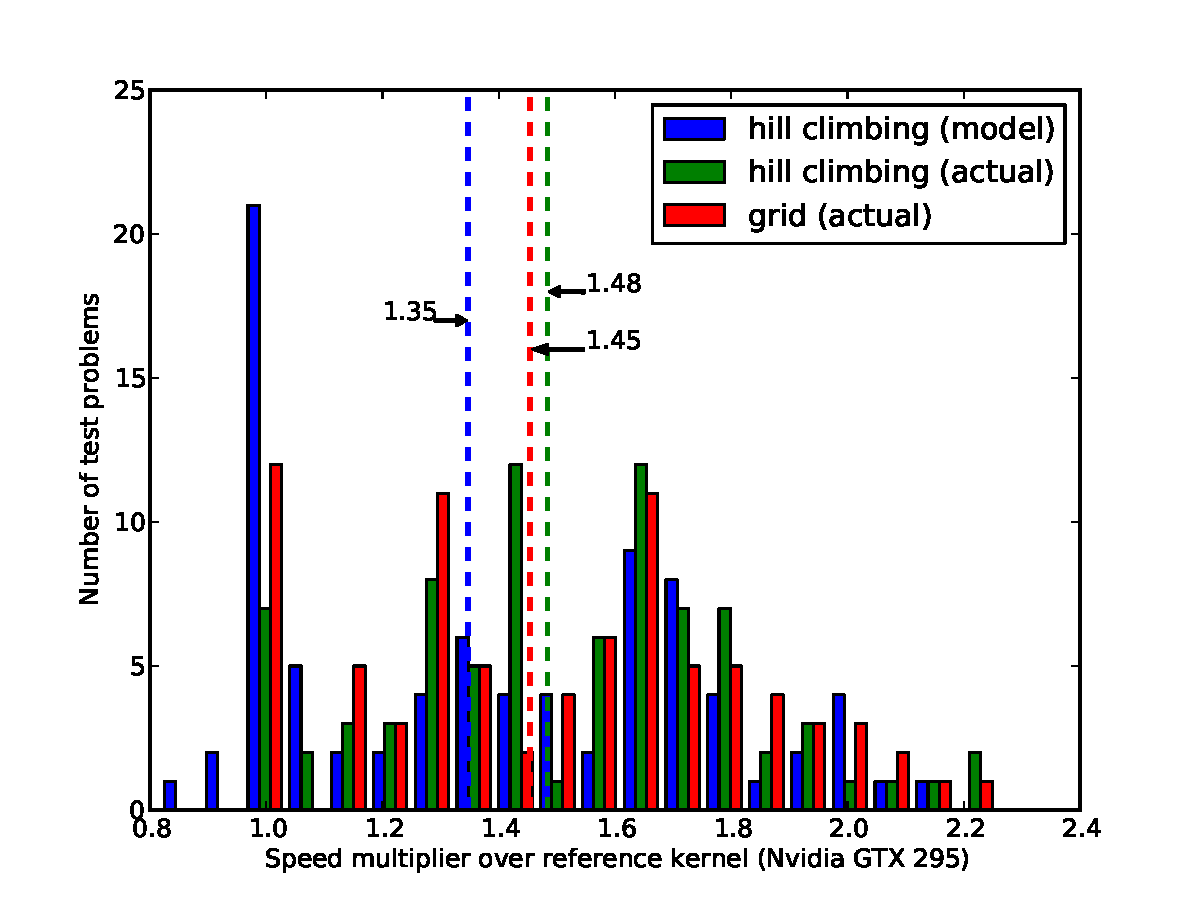
\includegraphics[scale=.42]{speedup_295.pdf}
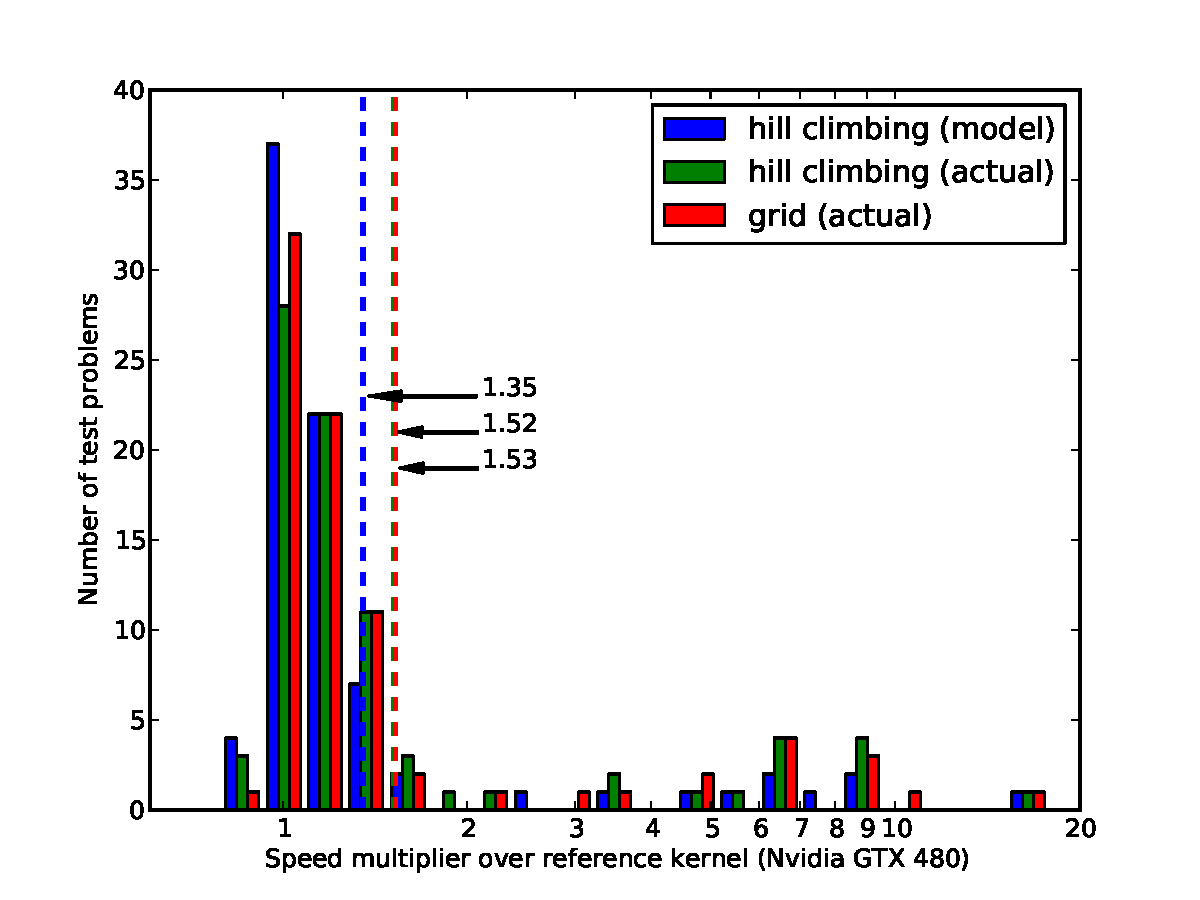
\includegraphics[scale=.42]{speedup_480.pdf}
\caption{Speedup of various auto-tuning strategies over a good reference
implementation.
Each strategy was evaluated the same set of 83 problem configurations, which
was disjoint from the problem configurations used to build the model for
model-based hill-climbing.
The vertical dashed lines are positioned at the geometric mean speedup (XXX?)
of each strategy. The grid and hill-climbing approaches
tested 73 and 75 configurations respectively, and took 45?? XXX
seconds on average.
The model-based approach tested 0 configuration evaluations, and took 0.05
seconds on average, even with a naive Python implementation.
}
\label{fig:speedup}
\end{figure*}


\begin{figure*}
\centering
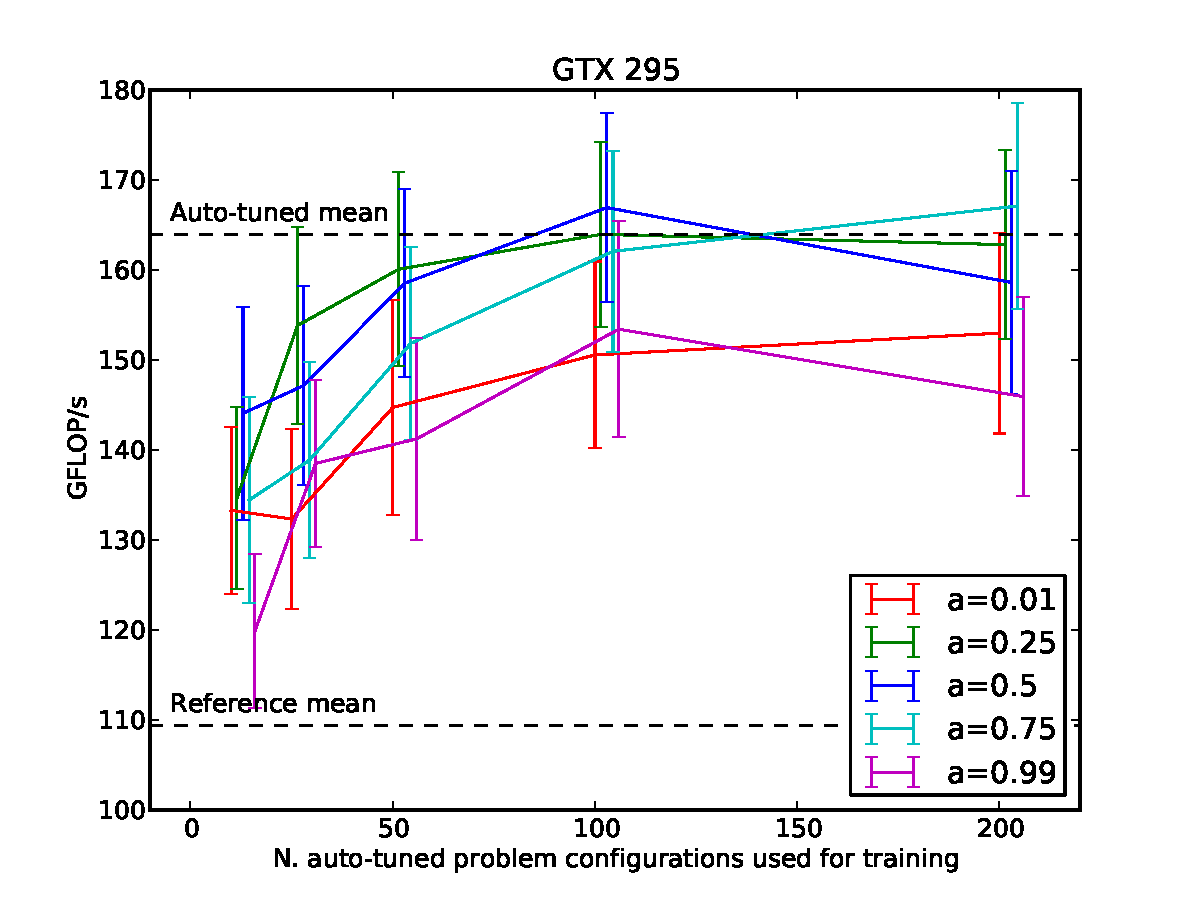
\includegraphics[scale=.42]{fig_ntrain_295.pdf}
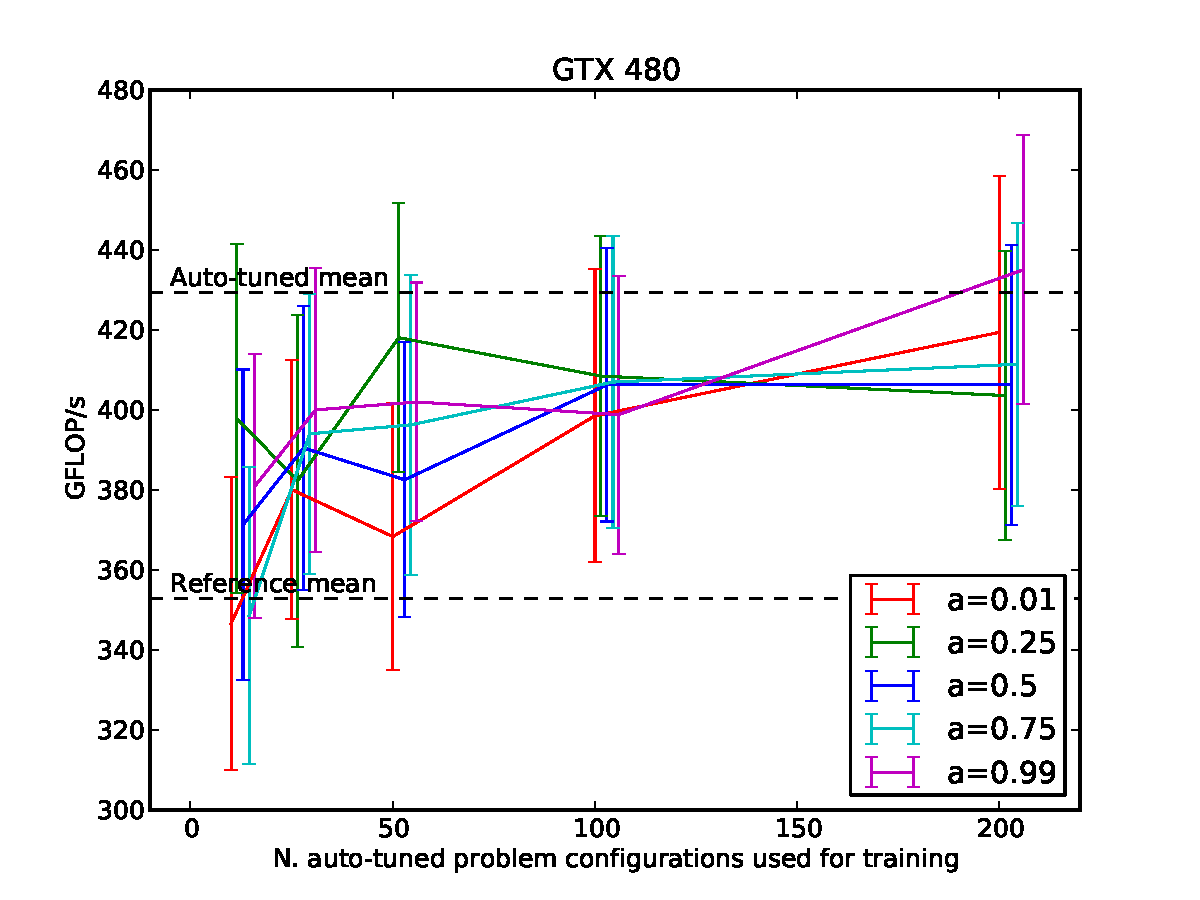
\includegraphics[scale=.42]{fig_ntrain_480.pdf}
\caption{The effect of the invalid configuration score ($a$) and training set
size on simulated auto-tuning.
All candidates timed during the grid and
hill-climbing search procedures were used as training points, so the training
set sizes ranged from an average of 1500 (10 problem configurations) to 30
thousand (200 problem configurations).
Training on 10 or 25 configurations was useful (higher mean than the reference),
but not as useful as training on 50 or more configurations.
The results on the GTX 295 suggest that
moderate values of $a$ between $0.25$ and $0.75$ might be
best, but $a$ had no significant effect on the GTX 480.
}
\label{fig:fig_ntrain}
\end{figure*}

\begin{figure*}
\centering
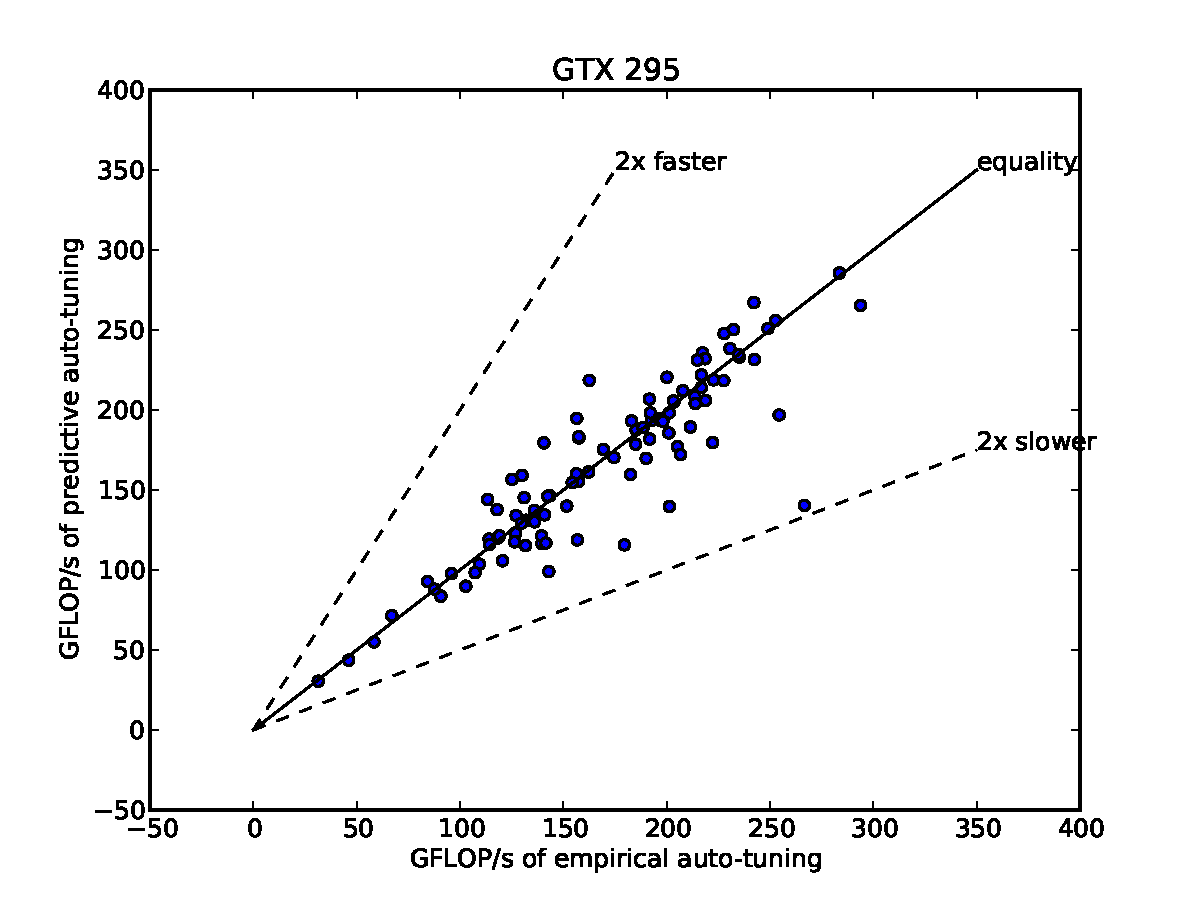
\includegraphics[scale=.42]{fig_gflop_scatter_295.pdf}
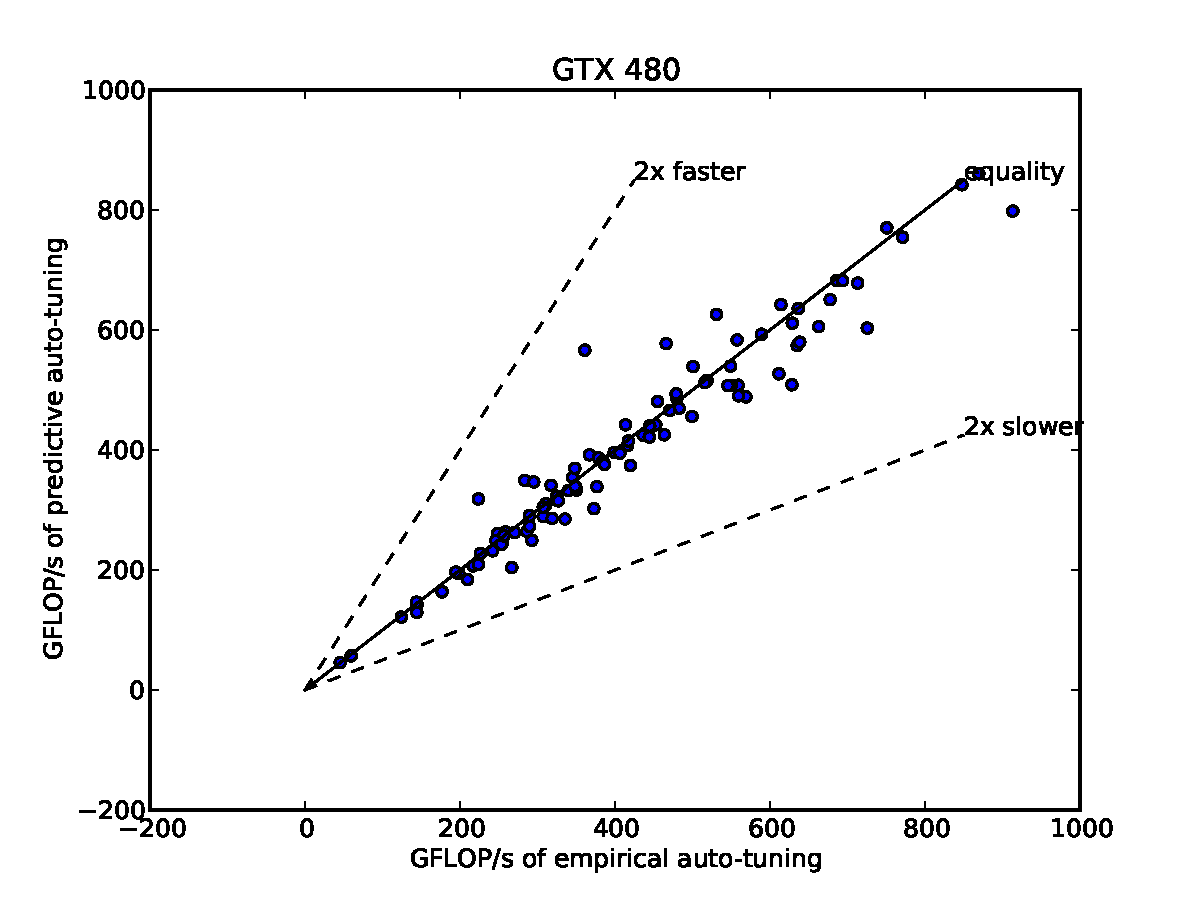
\includegraphics[scale=.42]{fig_gflop_scatter_480.pdf}
\caption{Computation speed for novel problem configurations using predictive
vs. empirical code specialization.
The scatterplots are roughly symmetric about the axis of equality (main diagonal)
with occasional outliers, indicating that for most problem configurations the
predictive approach gives as good a solution as the empirical approach.
The predictive approach typically requires about 0.1 seconds to suggest an
implementation, whereas the empirical approach requires about 2 minutes.
}
\label{fig:fig_gflop_scatter}
\end{figure*}

\subsection{Model-based Autotuning}

On the GTX 295, a single decision-tree fit to the log-speed-multiplier
(LSM) function (XXX: how many problem configurations, how much vs. what
kind of training data) achieves an average Spearman correlation of 0.9 on
held-out test data (XXX: what kind of test data).

Now: the big test is that if we use the genetic search on the model instead of
the original function, do we get good performance?

\section{Discussion}

We're characterizing hardware by a 1-of-N feature vector, simply describing
which hardware is the current hardware.
To make better use of auto-tuning data from other platforms, it would be more
useful to have precise and descriptive features such as: what compute
capability is present, how many cores are active, what is the bandwidth
between the various kinds of memory, and how much of various kinds of memory
is present.  With these features a model-assisted auto-tuning approach
might be able to make very good guesses on hardware for which no auto-tuning
has ever been done.

In a complete implementation of Eq.~\ref{eq:z}, there would be parameters
related to the physical layout (e.g. strides) of $x$, $f$ and $z$ arrays in
addition to the mathematical parameters of heights and widths and so on,
so the total number of filterbank correlation computations that a user might
be able to demand is astronomical.
A typical coping mechanism would be to cast an arbitrary problem configuration into a more
standardized form, such as by copying inputs into aligned memory buffers with
appropriate padding, and then choosing an appropriate blocking strategy for
the computation. At that point, auto-tuning efforts can be focussed on the
kernel for each blocked strategy. However, on GPU hardware, the cost of
aligning the inputs can be relatively large.  In future work we hope to apply
our model-based technique to auto-tune in full problem configuration space, so
that we can optimize as much of the computation as possible within the
predictive auto-tuning framework (XXX name).

Platform Space: XXX

XXX: GCG chapter pg 13 notes that among the grid search, the best parameter
setting is different for the various platforms.

XXX: so far we only tried 3 cards... so we're using a 1-of-N feature.


%\renewcommand{\bibsection}{\section*{Bibliography}}
%\setlength{\bibsep}{5pt}
\bibliography{local}
\end{document}
